\documentclass{ximera}

%% You can put user macros here
%% However, you cannot make new environments

\listfiles

\graphicspath{{./}{firstExample/}{secondExample/}}

\usepackage{tikz}
\usepackage{tkz-euclide}
\usepackage{tikz-3dplot}
\usepackage{tikz-cd}
\usetikzlibrary{shapes.geometric}
\usetikzlibrary{arrows}
\usetikzlibrary{decorations.pathmorphing,patterns}
\usetkzobj{all}
\pgfplotsset{compat=1.13} % prevents compile error.

\renewcommand{\vec}[1]{\mathbf{#1}}
\newcommand{\RR}{\mathbb{R}}
\newcommand{\dfn}{\textit}
\newcommand{\dotp}{\cdot}
\newcommand{\id}{\text{id}}
\newcommand\norm[1]{\left\lVert#1\right\rVert}
 
\newtheorem{general}{Generalization}
\newtheorem{initprob}{Exploration Problem}

\tikzstyle geometryDiagrams=[ultra thick,color=blue!50!black]

\usepackage{mathtools}

\title{Applications Leading to Differential Equations}


\begin{document}

\begin{abstract}
Need an abstract
\end{abstract}

\maketitle

\section*{Applications Leading to Differential Equations}

In order to apply mathematical methods to a physical or ``real life''
problem, we must  formulate the problem in mathematical
terms; that is, we must construct a {\color{blue}\it mathematical
model\/} for the
problem. Many physical problems concern relationships between changing
quantities. Since rates of change are represented mathematically by
derivatives, mathematical models often involve equations relating an
unknown function and one or more of its derivatives. Such equations
are  {\color{blue}\it differential equations}. They are the subject of this
book.

Much of calculus is devoted to learning mathematical techniques that
are applied in later courses in mathematics and the sciences;     you
wouldn't have time to learn much calculus if you insisted on seeing
a specific application of every topic covered in the course.
Similarly, much of this book is devoted to methods that can be applied
in later courses. Only a relatively small part of the book is devoted
to the derivation of specific differential equations from mathematical
models, or relating the differential equations that we study to
specific applications. In this section we mention a few such
applications.

The mathematical model for an applied problem is almost always simpler
than the actual situation being studied, since simplifying assumptions
are usually required to obtain a mathematical problem that can be
solved. For example, in modeling the motion of a falling object, we
might neglect air resistance and the gravitational pull of celestial
bodies other than Earth, or in  modeling  population growth we
might assume that the population grows continuously rather than in
discrete steps.

A good mathematical model has two important properties:

\begin{itemize}
\item It's sufficiently simple so that the mathematical problem
can be solved.

\item It represents the actual situation sufficiently well so that the
solution to the mathematical problem predicts the outcome of the real
problem to within a useful degree of accuracy. If results predicted by
the model don't agree with physical observations, the
underlying
assumptions of the model must be revised until satisfactory agreement
is obtained.
\end{itemize}

We'll  now give  examples of mathematical models involving
differential equations. We'll return to these problems at the
appropriate times, as we learn how to solve the various types of
differential equations that occur in the models.

All the examples in this section deal with functions of time, which we
 denote by $t$. If $y$ is a function of $t$,  $y'$
denotes the derivative of $y$ with respect to $t$;   thus,
$$
y'={dy\over dt}.
$$

\boxit{Population Growth and Decay}

\noindent
Although the number of members of a population (people in a given
country, bacteria in a laboratory culture, wildflowers in a forest,
etc.)
at any given time $t$ is necessarily an integer, models that use
differential equations to describe the growth and decay of populations
usually rest on the simplifying assumption that the number of members of
the population can be regarded as a differentiable function $P=P(t)$.
In most models it is assumed that the differential equation takes the
form
\begin{equation} \label{eq:1.1.1}
P'=a(P)P,
\end{equation}
where $a$ is a continuous function of $P$ that represents the rate of
change of population per unit time per individual.
In the
\href{http://en.wikipedia.org/wiki/Thomas_Robert_Malthus}
{\color{blue}\it Malthusian model},
 it is assumed that
$a(P)$ is a constant, so \eqref{eq:1.1.1} becomes
\begin{equation} \label{eq:1.1.2}
P'=aP.
\end{equation}
\color{blue}
(When you see a name in blue italics, just click on it for
information about the person.)
\color{black}
This model assumes that the numbers of births and deaths per unit time
are both proportional to the population. The constants of
proportionality are  the {\color{blue}\it birth rate\/} (births per unit
time per individual) and the {\color{blue}\it death rate\/} (deaths per unit time
per individual);     $a$ is the birth rate minus the death rate.
You  learned in calculus that if $c$ is any constant then
\begin{equation} \label{eq:1.1.3}
P=ce^{at}
\end{equation}
satisfies \eqref{eq:1.1.2}, so \eqref{eq:1.1.2} has infinitely
many solutions. To select the solution of the specific problem that
we're considering, we must know the population $P_0$ at an initial
time, say $t=0$. Setting $t=0$ in \eqref{eq:1.1.3} yields
$c=P(0)=P_0$, so the applicable solution is
$$
P(t)=P_0e^{at}.
$$
This implies that
$$
\lim_{t\to\infty}P(t)=\left\{\begin{array}{cl}\infty&\mbox{ if
}a>0,\\ 0&\mbox{ if }a<0;    \end{array}\right.
$$
that is, the population approaches infinity if the birth rate exceeds
the death rate, or zero if the death rate exceeds the birth rate.

To see the limitations of the Malthusian model, suppose  we're
modeling the  population of a country, starting from a time
$t=0$ when the birth rate exceeds the death rate (so $a>0$), and
the country's resources in terms of space, food supply, and other
necessities of life can support the existing population. Then the
prediction $P=P_0e^{at}$ may be reasonably accurate as long as
it remains within limits that the country's resources can support.
However, the model must inevitably lose validity when the prediction
exceeds these limits. (If nothing else, eventually there won't be
enough space for the predicted population!)

This flaw in the Malthusian model suggests the need for a model that
accounts for limitations of space and resources that tend to oppose
the rate of population growth as the population increases.
 Perhaps the most famous model of this kind is the
\href{http://www-history.mcs.st-and.ac.uk/Mathematicians/Verhulst.html}
{\color{blue}\it Verhulst
 model\/}, where \eqref{eq:1.1.2} is
replaced by
\begin{equation} \label{eq:1.1.4}
P'=aP(1-\alpha P),
\end{equation}
where $\alpha$ is a positive constant.
As long as $P$ is small
compared to $1/\alpha$, the ratio $P'/P$  is approximately equal to $a$.
Therefore the growth is approximately exponential;     however, as $P$
increases, the ratio $P'/P$  decreases as opposing factors
become significant.

Equation~\eqref{eq:1.1.4} is  the {\color{blue}\it logistic equation\/}. You
will learn how to solve it in Section~1.2. (See
Exercise~2.2.~\hspace*{-3pt}\ref{exer:2.2.28}.) The solution is
$$
P={P_0\over\alpha P_0+(1-\alpha P_0)e^{-at}},
$$
where $P_0=P(0)>0$. Therefore
$\lim_{t\to\infty}P(t)=1/\alpha$, independent of $P_0$.

Figure~\ref{figure:1.1.1} shows typical graphs of $P$ versus $t$ for
various values of  $P_0$.

\begin{figure}[h]
  \centering
  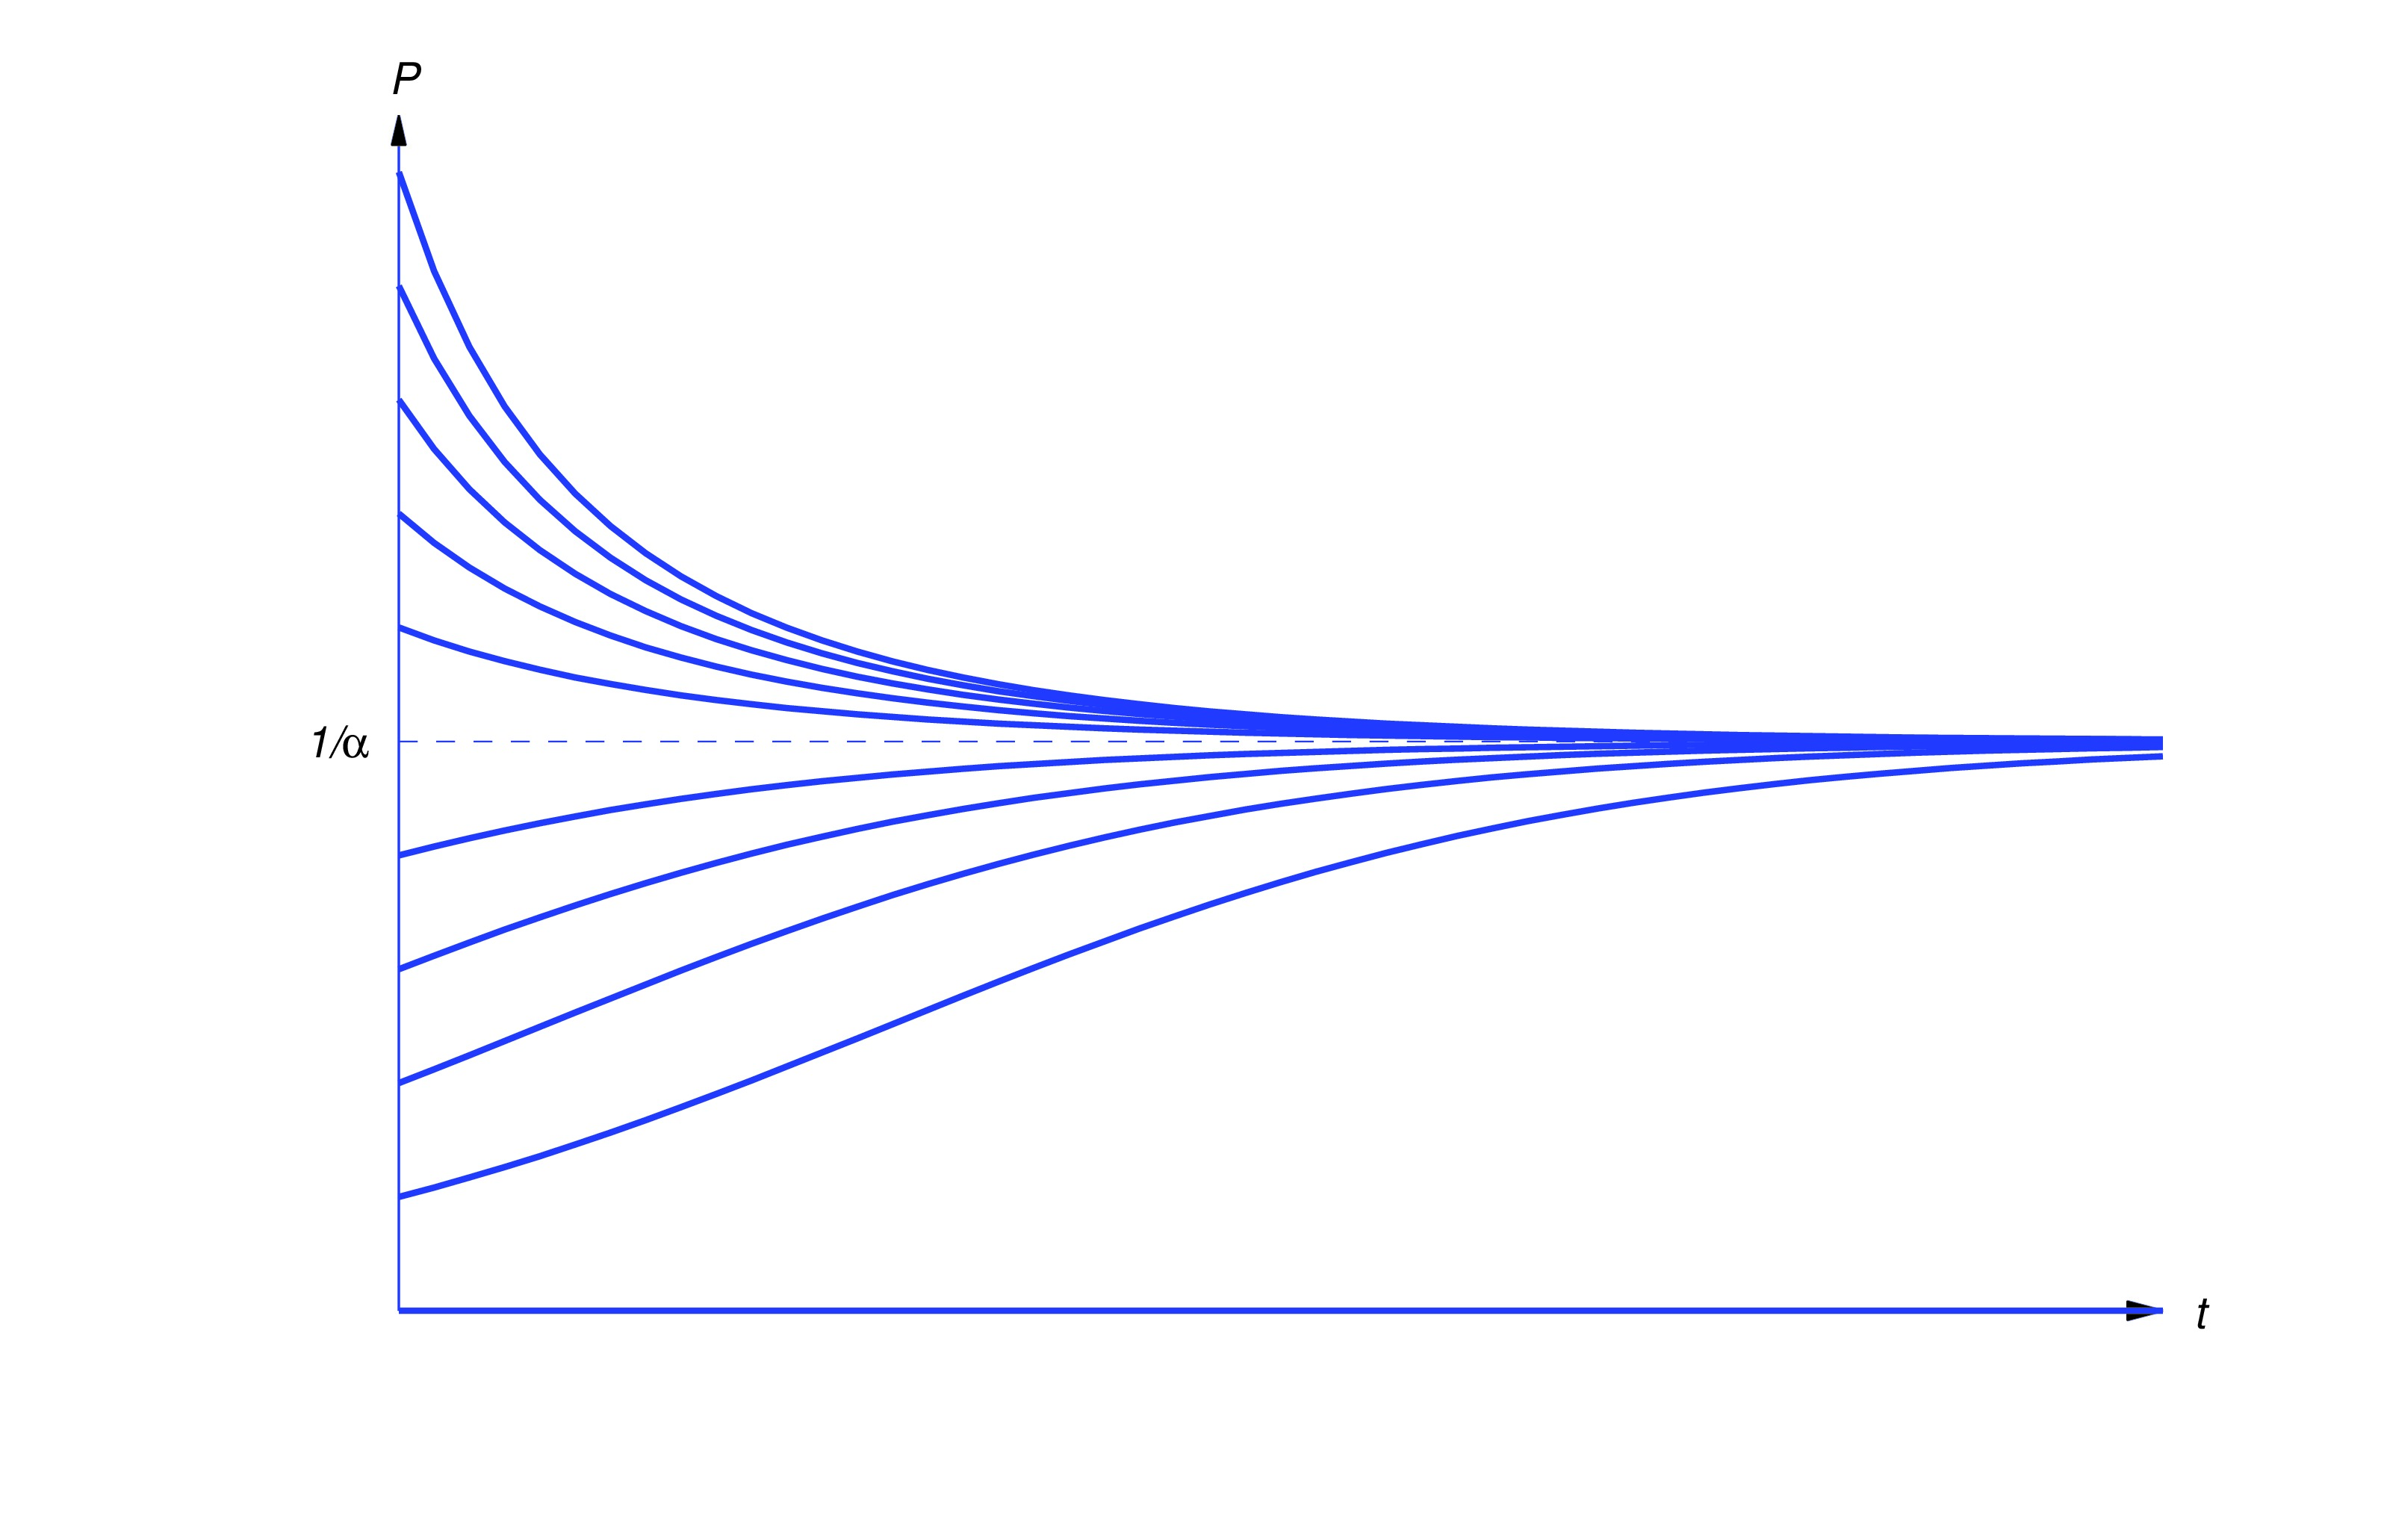
\includegraphics[bb=-78 148 689 643,width=5.67in,height=3.66in,keepaspectratio]{fig010101}
\color{blue}
  \caption{ Solutions of the logistic equation}
  \label{figure:1.1.1}
\end{figure}


\boxit{Newton's Law of Cooling}

\noindent
According to
\href{http://www-history.mcs.st-and.ac.uk/Mathematicians/Newton.html}
{\color{blue}\it Newton's
law of cooling},  the temperature of a
body changes at a rate proportional to the difference between the
temperature of the body and the temperature of the surrounding medium.
 Thus, if  $T_m$ is the temperature of the
medium and
$T=T(t)$ is the temperature of the body at time $t$, then
\begin{equation} \label{eq:1.1.5}
T' = -k(T-T_m),
\end{equation}
where $k$ is a positive constant and the  minus sign indicates;   that
the temperature of the body increases with time if it's less than the
temperature of the medium, or decreases if it's  greater. We'll see
in Section~4.2 that if
$T_m$ is constant then the solution of \eqref{eq:1.1.5} is
\begin{equation} \label{eq:1.1.6}
T=T_m+(T_0-T_m)e^{-kt},
\end{equation}
where $T_0$ is the temperature of the body when $t=0$.
Therefore $\lim_{t\to\infty}T(t)=T_m$, independent of $T_0$.
(Common sense suggests this. Why?)

Figure~\ref{figure:1.1.2} shows typical graphs of $T$ versus $t$ for
various values of  $T_0$.

\begin{image}
{\def\length{sqrt(1+(x+y)^2)}
\begin{tikzpicture}
  \begin{axis}
  [      xmin=-1, xmax=10,ymin=-1,ymax=8,domain=0:10,view={0}{90},
      axis lines =center, xlabel=$t$, ylabel=$T$, ticks=none
      ]
    \addplot[penColor,very thick]{3+3*e^(-0.5*x)};
    \addplot[penColor,very thick]{3+2*e^(-0.5*x)};
    \addplot[penColor,very thick]{3+e^(-0.5*x)};
    \addplot[penColor,very thick]{3-e^(-0.5*x)};
    \addplot[penColor,very thick]{3-2*e^(-0.5*x)};
    \addplot[penColor,very thick]{3-3*e^(-0.5*x)};
    \addplot[penColor,dashed]{3};
    
    \node[] at (-0.5, 3)  (r3)    {$T_m$};
\end{axis}
\end{tikzpicture}}
\end{image}

Assuming that the medium remains at constant temperature seems
reasonable if we're considering a cup of coffee cooling in a room, but
 not if we're cooling a huge cauldron of molten
metal in the same room. The difference between the two situations is
that the heat lost by the coffee isn't likely to raise the
temperature of the room appreciably, but the heat lost by the
cooling metal is. In this second situation we must use a model that
accounts for the heat exchanged between the object and the medium. Let
$T=T(t)$ and $T_m=T_m(t)$ be the temperatures of the object and the
medium respectively, and let $T_0$ and $T_{m0}$ be their initial
values. Again, we assume that $T$ and $T_m$ are related by
\eqref{eq:1.1.5}. We also assume that the change in heat of
the object as its temperature changes from $T_0$ to $T$ is $a(T-T_0)$
and  the change in heat of the medium as its temperature changes
from $T_{m0}$ to $T_m$ is $a_m(T_m-T_{m0})$, where $a$ and $a_m$ are
positive constants depending upon the masses and thermal properties of
the object and medium respectively. If we assume that the total heat
of the in the object and the medium remains constant
(that is, energy is conserved), then
$$
a(T-T_0)+a_m(T_m-T_{m0})=0.
$$
Solving this for  $T_m$  and substituting the result into
\eqref{eq:1.1.6} yields the differential equation
$$
T'=-k\left(1+{a\over a_m}\right)T
+k\left(T_{m0}+{a\over a_m}T_0\right)
$$
for the temperature of the object.  After learning to solve linear
first order  equations, you'll be able to show
(Exercise~4.2.~\hspace*{-3pt}\ref{exer:4.2.17}) that
$$
T={aT_0+a_mT_{m0}\over
a+a_m}+{a_m(T_0-T_{m0})\over a+a_m}e^{-k(1+a/a_m)t}.
$$

\boxit{Glucose Absorption by the Body}

\noindent
Glucose is absorbed by
the body at a rate proportional to the amount of glucose present in
the bloodstream. Let $\lambda$ denote the (positive) constant of
proportionality. Suppose   there are $G_0$ units of glucose in
the bloodstream when $t=0$, and let $G=G(t)$ be the number of units in
the bloodstream at time $t>0$. Then, since the glucose being absorbed
by the body is leaving the bloodstream, $G$ satisfies the equation
\begin{equation} \label{eq:1.1.7}
G'=-\lambda G.
\end{equation}
From  calculus you know that if $c$ is any constant then
\begin{equation} \label{eq:1.1.8}
G=ce^{-\lambda t}
\end{equation}
satisfies \eqref{eq:1.1.7}, so \eqref{eq:1.1.7} has infinitely
many solutions.
 Setting $t=0$ in \eqref{eq:1.1.8} and requiring that
$G(0)=G_0$ yields $c=G_0$, so
$$
G(t)=G_0e^{-\lambda t}.
$$

Now let's complicate matters by injecting glucose intravenously
at a constant rate of $r$ units of glucose per unit of time.
Then the rate of change of the amount of glucose  in the bloodstream
per unit time is
\begin{equation} \label{eq:1.1.9}
G'=-\lambda G+r,
\end{equation}
where the first term on the right is due to the absorption of the
glucose by the body and the second term is due to the injection.
 After you've studied Section~2.1,
you'll be able to show (Exercise~2.1.~\hspace*{-3pt}\ref{exer:2.1.43}) that the solution
of
\eqref{eq:1.1.9} that satisfies $G(0)=G_0$ is
$$
G={r\over\lambda}+\left(G_0-{r\over\lambda}\right)e^{-\lambda t}.
$$
Graphs of  this function are similar to those in
Figure~\ref{figure:1.1.2}.
(Why?)

\boxit{Spread of Epidemics}

\noindent
One model for the spread of epidemics assumes that the number of
people infected changes at a rate proportional to the product of the
number of people already infected and the number of people who are
susceptible, but not yet infected. Therefore, if $S$ denotes the
total population of susceptible people and $I=I(t)$ denotes the
number
of infected people at time $t$, then $S-I$ is the number of people
who are susceptible, but not yet infected. Thus,
$$
I'=rI(S-I),
$$
where $r$ is a positive constant. Assuming that $I(0)=I_0$,
the solution of this equation is
$$
I={SI_0\over I_0+(S-I_0)e^{-rSt}}
$$
(Exercise~2.2.~\hspace*{-3pt}\ref{exer:2.2.29}).
 Graphs of this function are similar to those in
Figure~\ref{figure:1.1.1}.
(Why?)
Since $\lim_{t\to\infty}I(t)=S$, this model predicts that all the
susceptible people eventually become infected.

\boxit{Newton's Second Law of Motion}

\noindent

According to
\href{http://www-history.mcs.st-and.ac.uk/Mathematicians/Newton.html}
{\color{blue}\it Newton's second law of motion},  the
instantaneous acceleration
$a$ of an object with constant mass $m$ is related to the force $F$
acting on the object by the equation $F=ma$. For simplicity, let's
assume that $m=1$ and the motion of the object is along a vertical
line. Let $y$ be the displacement of the object from some reference
point on Earth's surface, measured positive upward. In many
applications, there are three kinds of forces that may act on the
object:

\begin{alist}
\item % (a)
A force such as gravity that depends only on the position $y$,
which we write as $-p(y)$, where $p(y)>0$ if $y\ge0$.

\item % (b)
A force such as atmospheric resistance that depends on
the position and velocity of the object, which we write as
$-q(y,y')y'$, where $q$ is a nonnegative function and we've
put $y'$ ``outside'' to indicate that the resistive force is
always in the direction opposite to the velocity.
\item % (c)
A force $f=f(t)$, exerted from an external source (such as a towline
from a helicopter) that depends only on $t$.
\end{alist}

In this case, Newton's second law implies that
$$
y''=-q(y,y')y'-p(y)+f(t),
$$
which is usually rewritten as
$$
y''+q(y,y')y'+p(y)=f(t).
$$
Since the  second (and no higher) order derivative of $y$ occurs in
this equation, we say that it is a {\color{blue}\it second order differential
equation\/}.

\boxit{Interacting Species: Competition}

\noindent
Let $P=P(t)$ and $Q=Q(t)$ be the populations of two species at time
$t$, and assume that each population would grow exponentially if the
other didn't exist; that is, in the absence of competition we would
have
\begin{equation} \label{eq:1.1.10}
P'=aP \mbox{\quad and \quad}Q'=bQ,
\end{equation}
where $a$ and $b$ are positive constants. One way to model the effect
of competition is to assume that the growth rate per individual of
each population is reduced by an amount proportional to the other
population, so \eqref{eq:1.1.10} is replaced by
\begin{eqnarray*}
P'&=&\phantom{-}aP-\alpha Q\\
Q'&=&-\beta P+bQ,
\end{eqnarray*}
where $\alpha$ and $\beta$ are positive constants. (Since negative
population doesn't make sense, this system works only while $P$ and
$Q$ are both positive.) Now suppose   $P(0)=P_0>0$ and
$Q(0)=Q_0>0$. It can be shown (Exercise~10.4.~\hspace*{-3pt}\ref{exer:10.4.42})
that there's a  positive constant $\rho$ such that if
$(P_0,Q_0)$ is above the line $L$ through the origin with slope $\rho$,
then the species with population $P$ becomes extinct in finite time,
but if $(P_0,Q_0)$ is below $L$,   the species with population
$Q$ becomes extinct in finite time. Figure~\ref{figure:1.1.3} illustrates
this. The curves shown there are given parametrically by $P=P(t),
Q=Q(t),\ t>0$.
 The arrows indicate direction along the curves with
increasing $t$.

\begin{figure}[h]
  \centering
  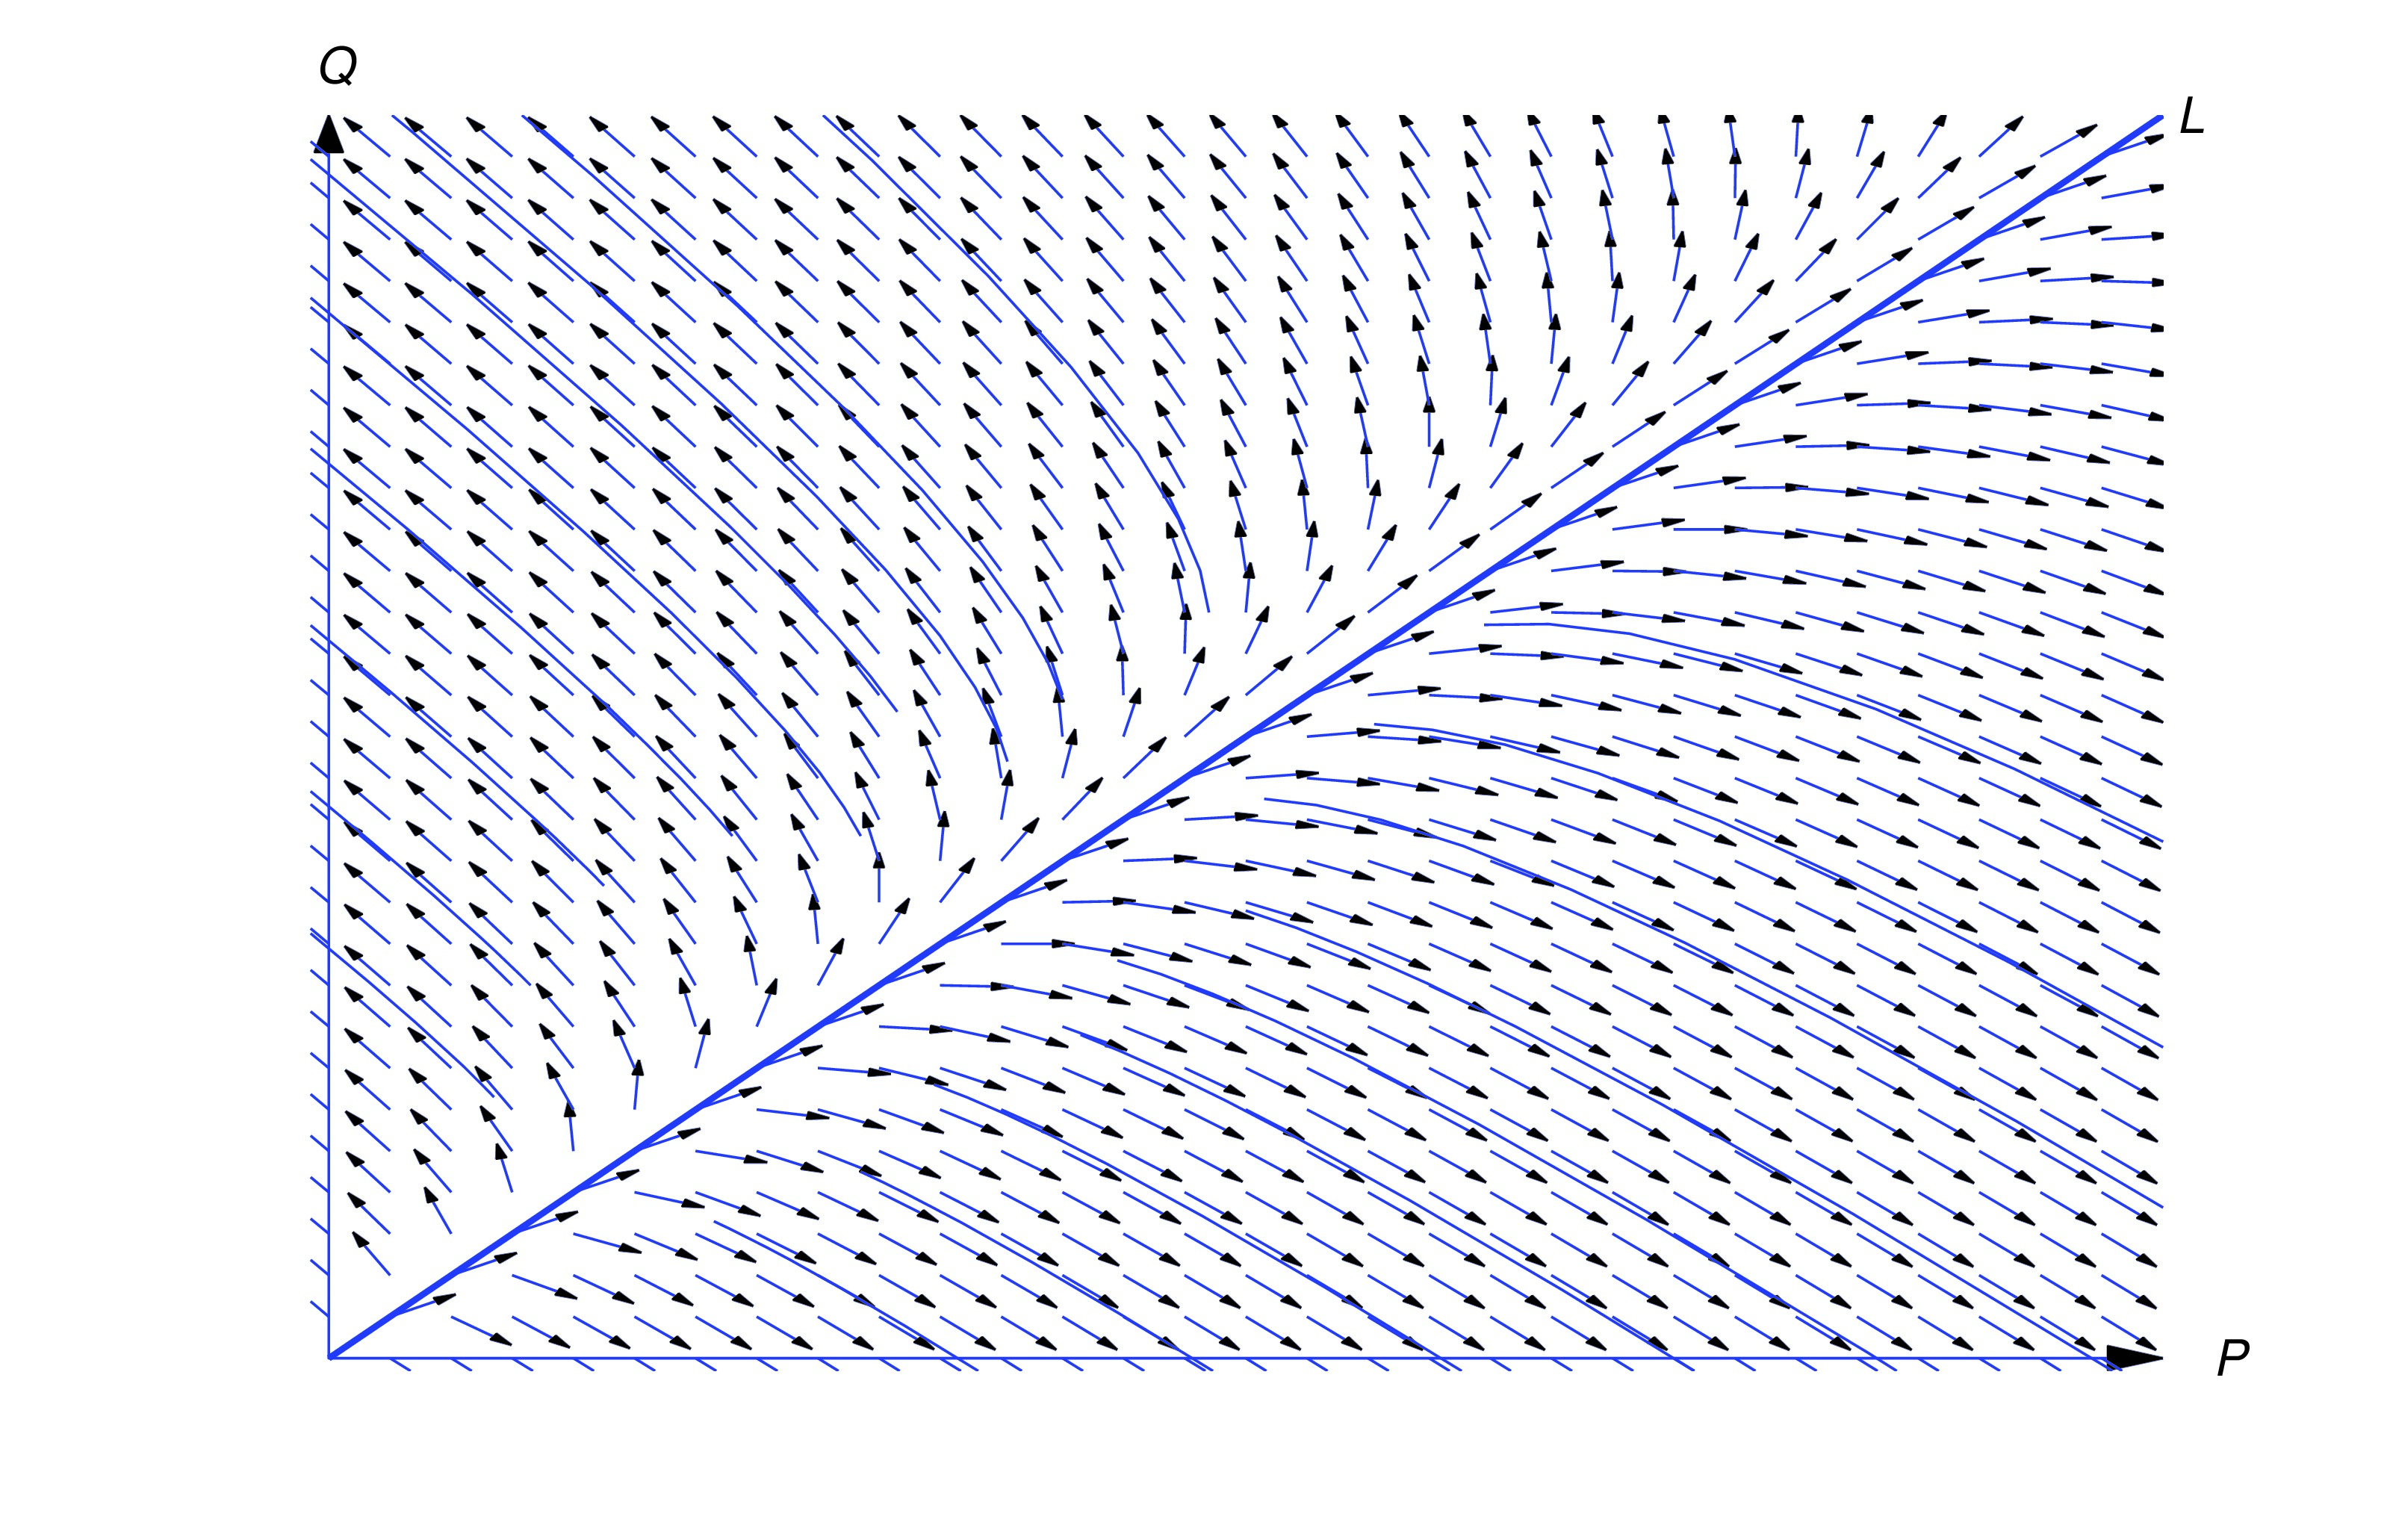
\includegraphics[bb=-78 148 689 643,width=5.67in,height=3.66in,keepaspectratio]{fig010103}
\color{blue}
  \caption{ Populations of competing species}
  \label{figure:1.1.3}
\end{figure}




\end{document}